\newpage
\addcontentsline{toc}{chapter}{Statement of Originality}

\begin{StatementofOriginality}

% 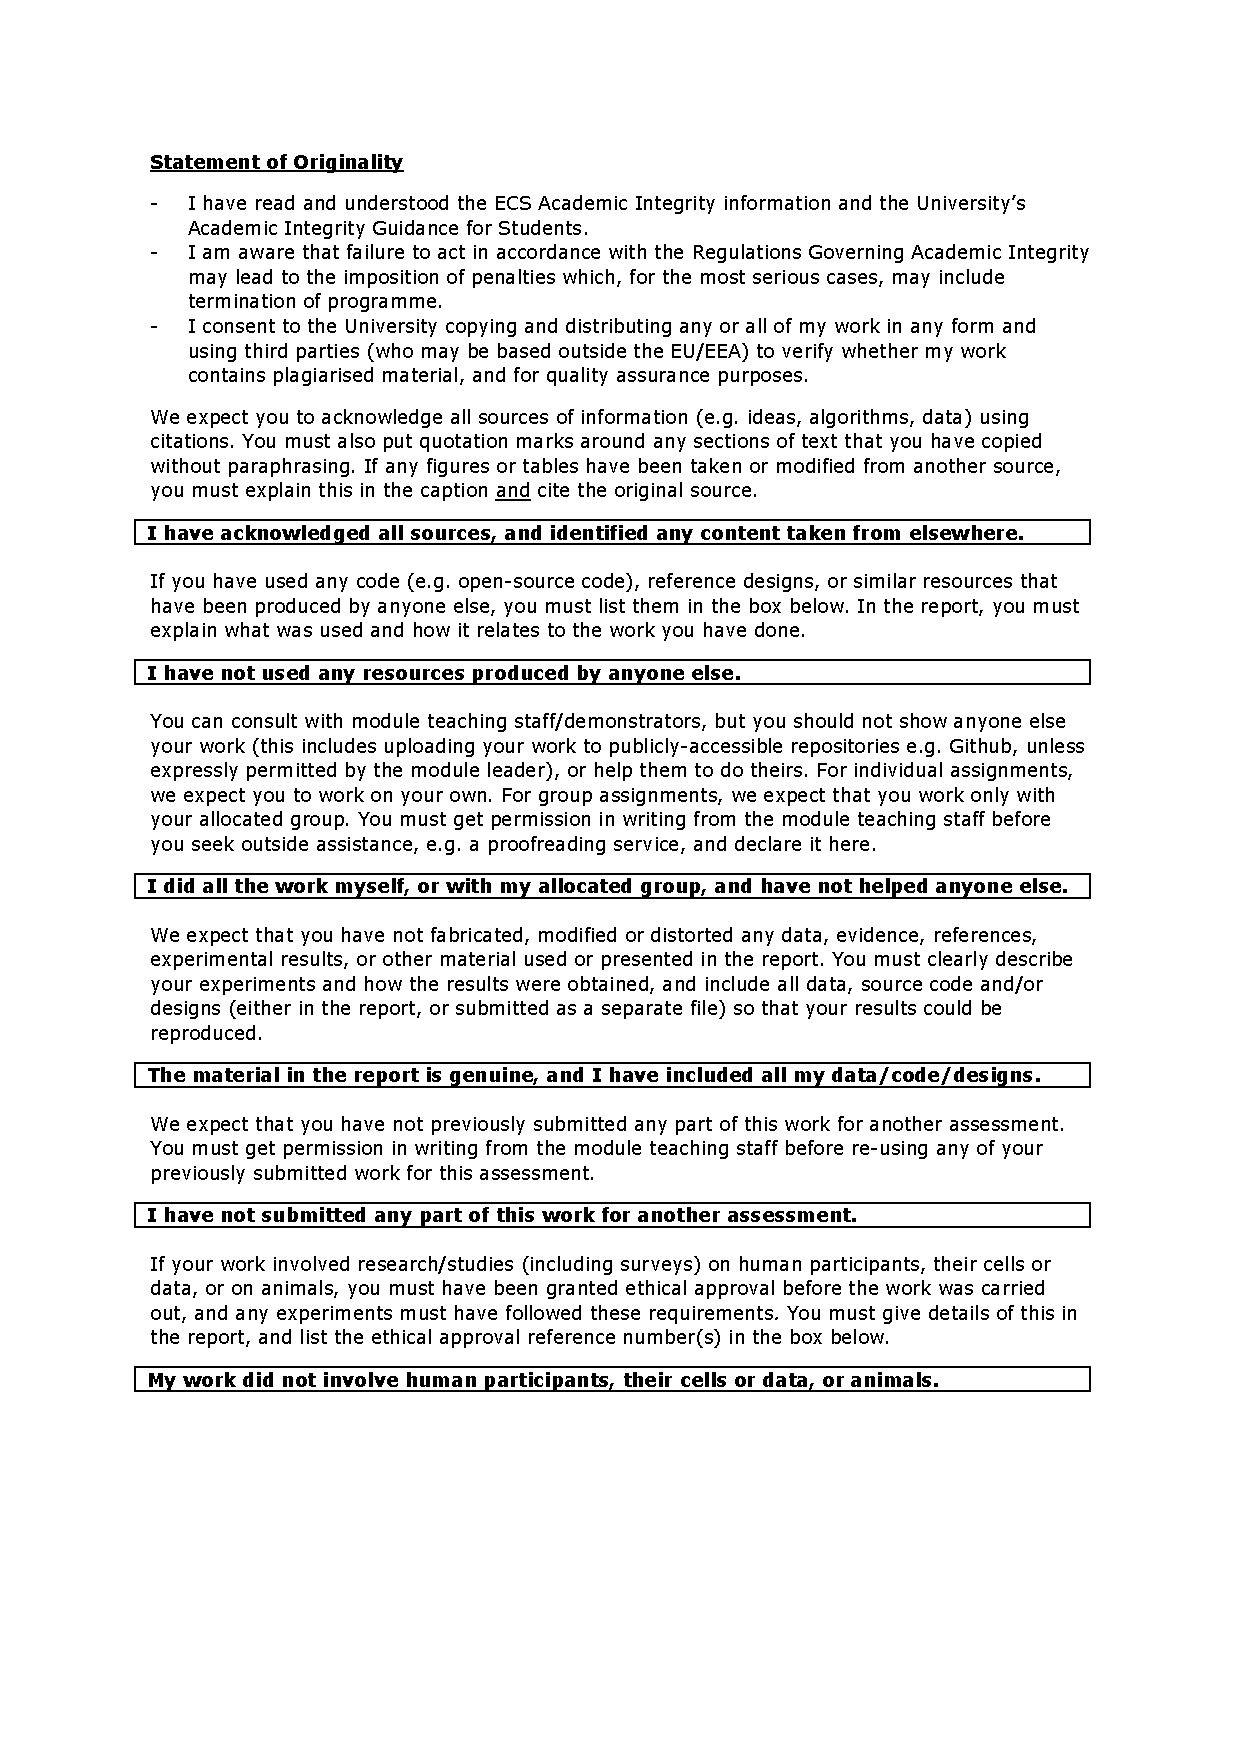
\includepdf[pages=+,noautoscale=true,offset=0 200, scale=0.7]{images/ai_statement.pdf}
% 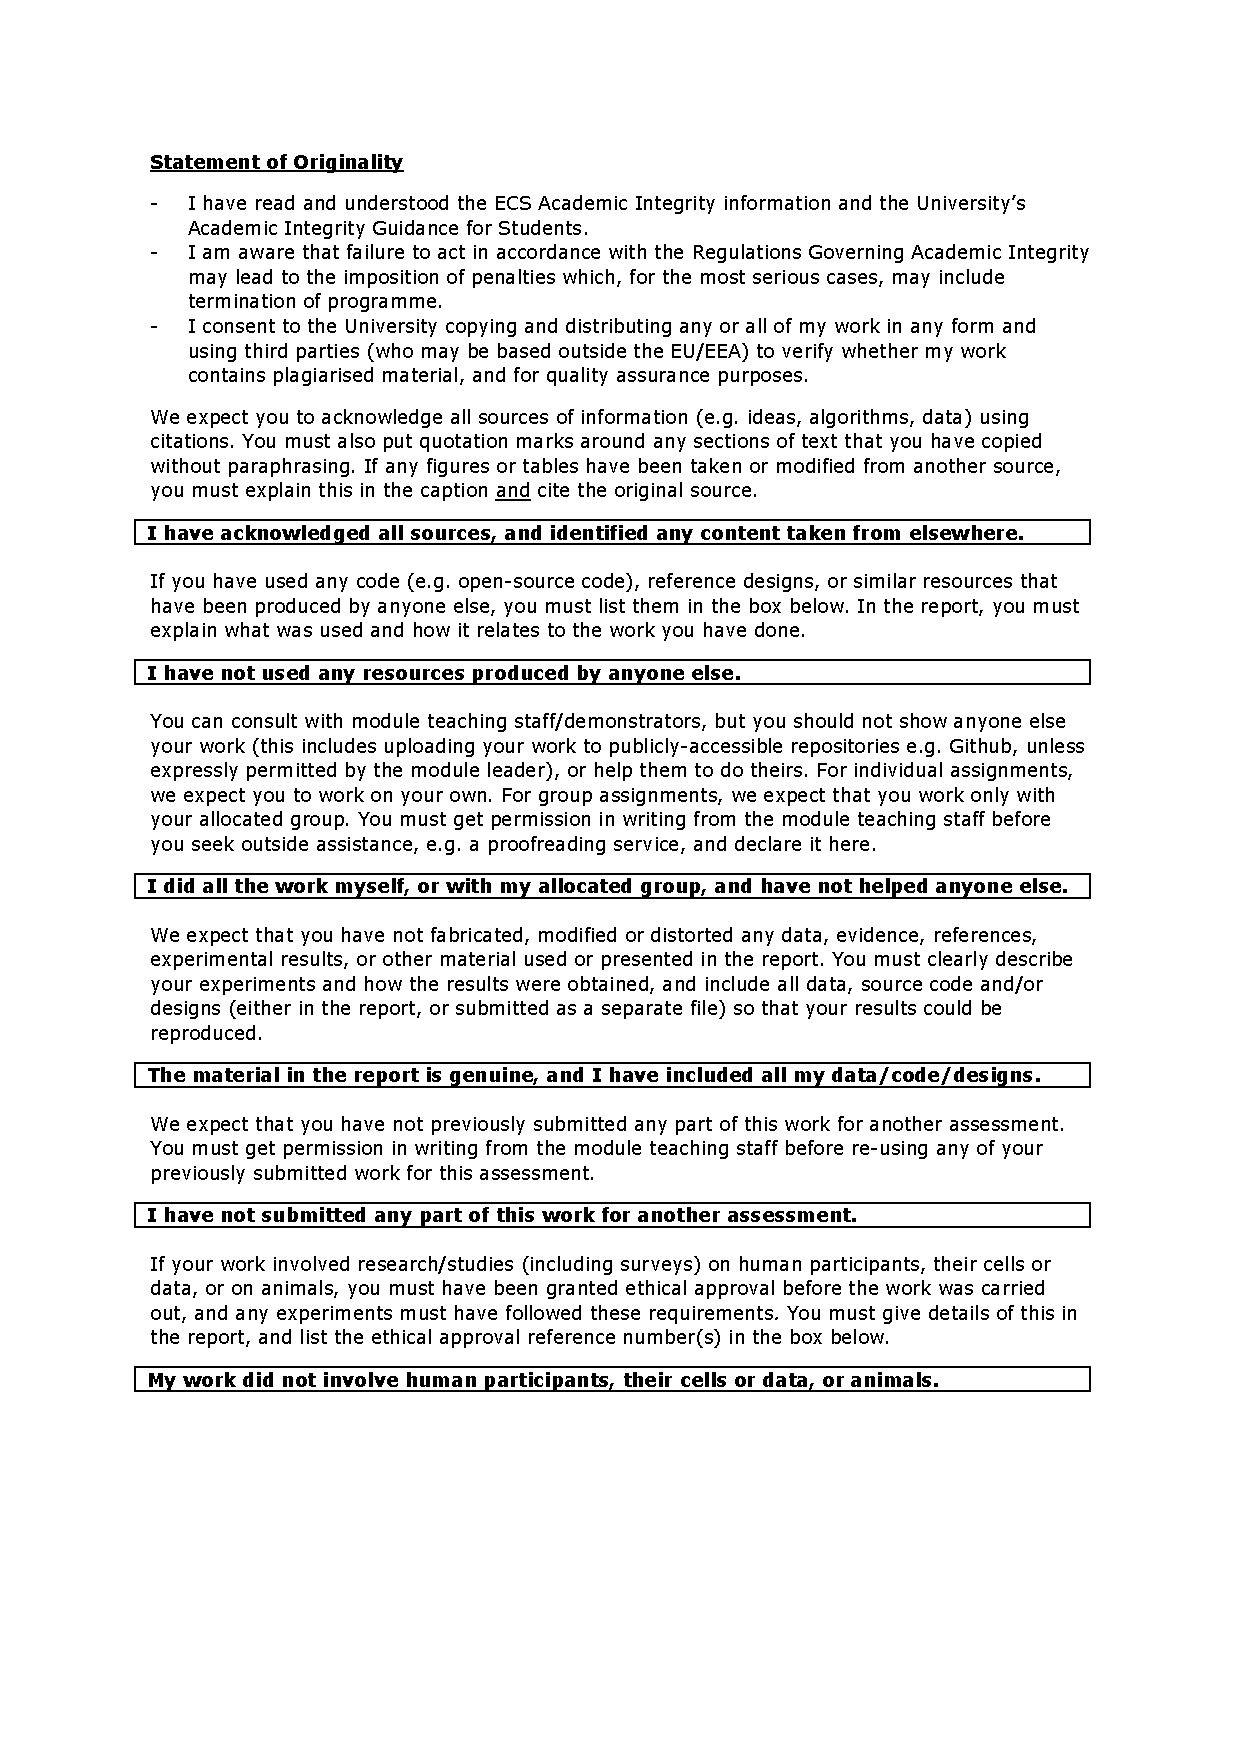
\includepdf[scale=0.5,pages=1,pagecommand={}]{images/ai_statement.pdf}

%\StatementofOriginality{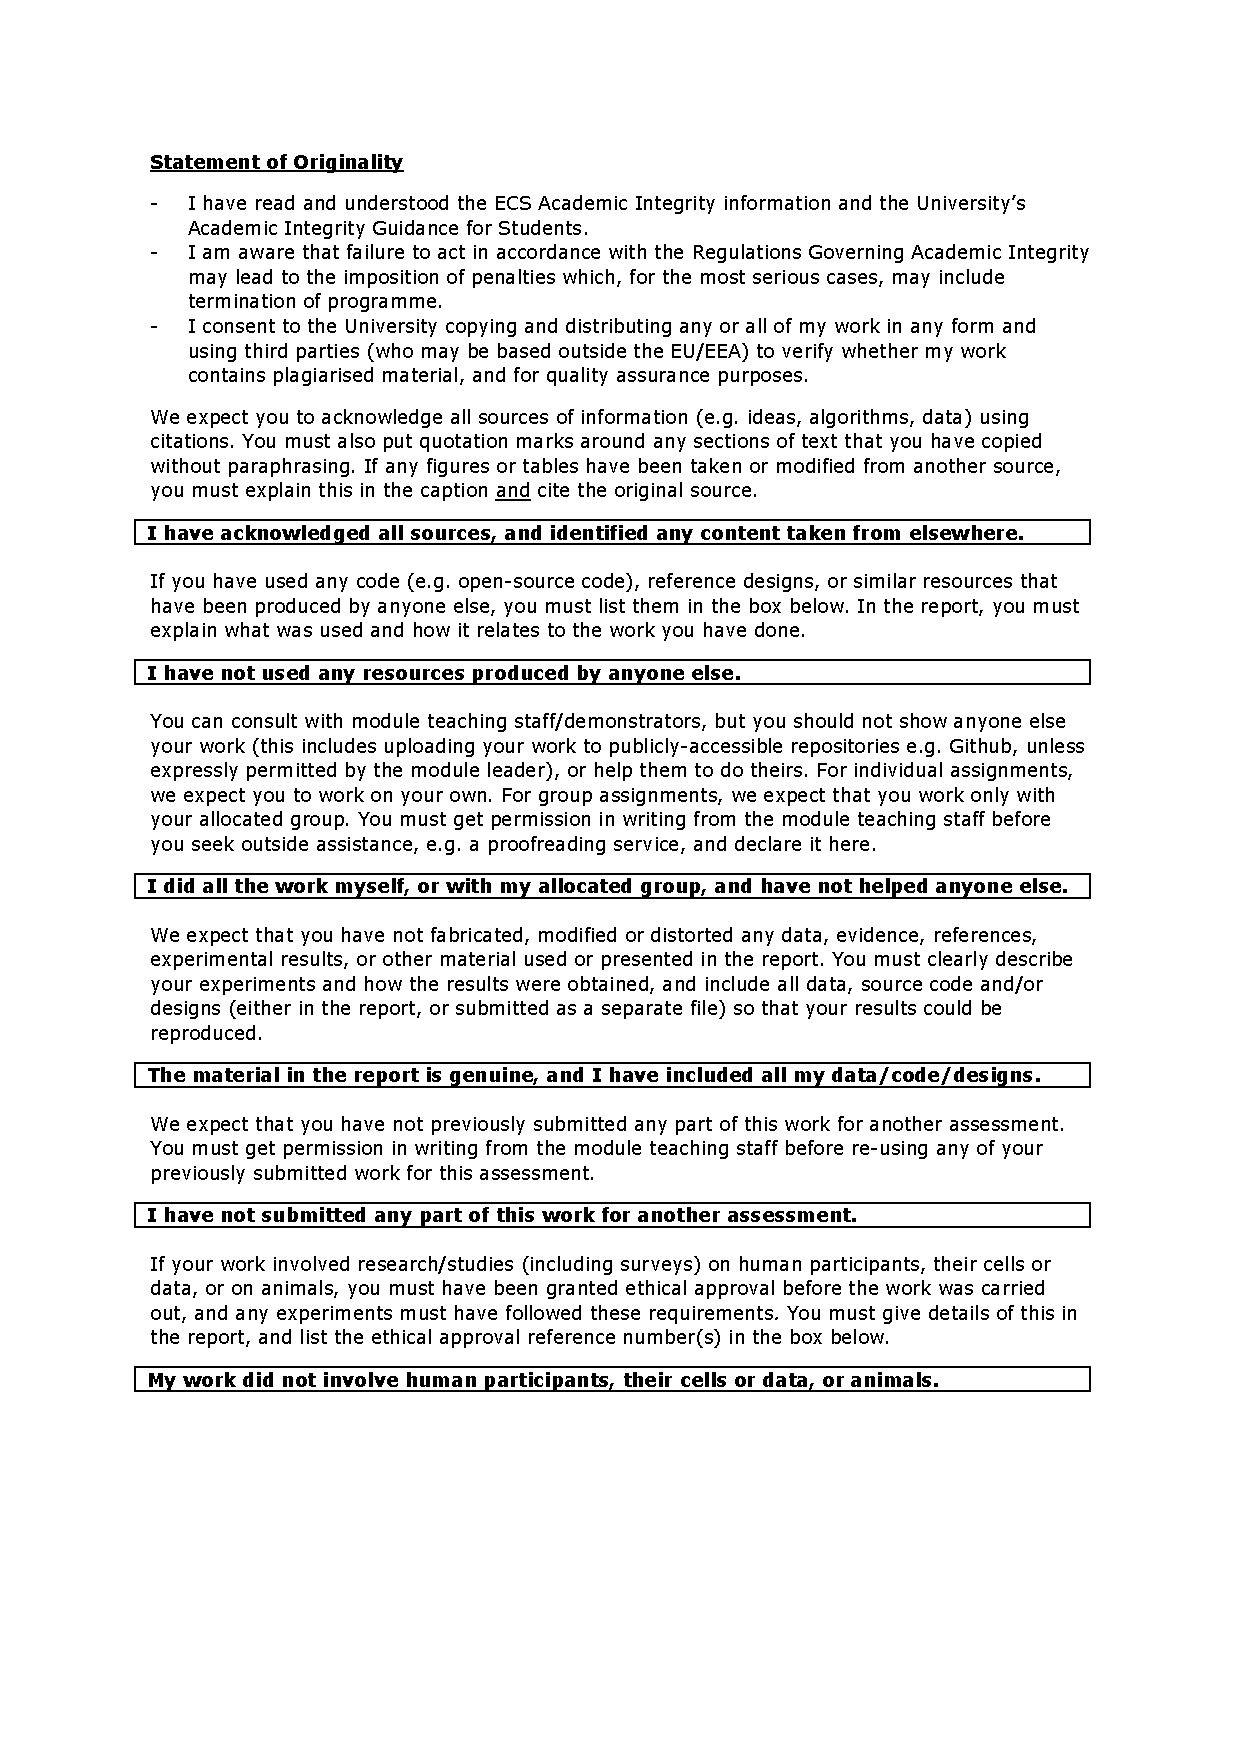
\includepdf[page=1,noautoscale=true, scale=1]{images/ai_statement.pdf}}

\begin{itemize}
\item[--] I have read and understood the ECS Academic Integrity information and the University's Academic Integrity Guidance for Students.
\item[--] I am aware that failure to act in accordance with the Regulations Governing Academic Integrity may lead to the imposition of penalties which, for the most serious cases, may include termination of programme.
\item[--]  I consent to the University copying and distributing any or all of my work in any form and using third parties (who may be based outside the EU/EEA) to verify whether my work contains plagiarised material, and for quality assurance purposes.
\end{itemize}
 
% We expect you to acknowledge all sources of information (e.g. ideas, algorithms, data) using citations. You must also put quotation marks around any sections of text that you have copied without paraphrasing. If any figures or tables have been taken or modified from another source, you must explain this in the caption and cite the original source. 
% I acknowledged all sources of information (e.g. ideas, algorithms, data) using citations. I also put quotation marks around any sections of text that I have copied without paraphrasing. When any figures or tables have been taken or modified from another source, I explained this in the caption and cited the original source. 
\vskip10pt

\begin{tcolorbox}
I have acknowledged all sources, and identified any content taken from elsewhere.
\end{tcolorbox}

\vskip20pt
% If you have used any code (e.g. open-source code), reference designs, or similar resources that have been produced by anyone else, you must list them in the box below. In the report, you must explain what was used and how it relates to the work you have done.
\begin{tcolorbox}
During the course of this project I followed different online tutorials and courses. All of them have been have been acknowledged in the body of the report and referenced in the bibliography (such as: \cite{projector}, \cite{whiteboard}, \cite{game1}, \cite{android}, \cite{visiongame}). Any minor additional source used, has been acknowledged in the code files available in the Project Design Archive as a comment. 
\end{tcolorbox}

\vskip20pt
% You can consult with module teaching staff/demonstrators, but you should not show anyone else your work (this includes uploading your work to publicly-accessible repositories e.g. Github, unless expressly permitted by the module leader), or help them to do theirs. For individual assignments, we expect you to work on your own. For group assignments, we expect that you work only with your allocated group. You must get permission in writing from the module teaching staff before you seek outside assistance, e.g. a proofreading service, and declare it here.

\begin{tcolorbox}
I did all the work myself and I have not helped anyone else.
\end{tcolorbox}

\vskip20pt
% We expect that you have not fabricated, modified or distorted any data, evidence, references, experimental results, or other material used or presented in the report. You must clearly describe your experiments and how the results were obtained, and include all data, source code and/or designs (either in the report, or submitted as a separate file) so that your results could be reproduced. 

\begin{tcolorbox}
The material in the report is genuine, and I have included all my data/code/designs.
\end{tcolorbox}

\vskip20pt

% We expect that you have not previously submitted any part of this work for another assessment. You must get permission in writing from the module teaching staff before re-using any of your previously submitted work for this assessment.

\begin{tcolorbox}
I have not submitted any part of this work for another assessment.
\end{tcolorbox}

% If your work involved research/studies (including surveys) on human participants, their cells or data, or on animals, you must have been granted ethical approval before the work was carried out, and any experiments must have followed these requirements. You must give details of this in the report, and list the ethical approval reference number(s) in the box below.
\begin{tcolorbox}
My work received ethical approval from the University of Southampton Ethics Committee. My application for Secondary Data Analysis has been sent through the ERGO \RNum{2} portal and is available in Appendix F (Submission ID = 48201, Category D). This application was necessary to carry out the data-sets exploration related to this project.
\end{tcolorbox}

\end{StatementofOriginality}